\documentclass[fr]{../../../../../../eplexam}

\hypertitle{Réseaux informatiques}{5}{INGI}{1341}{2020}{Janvier}{All}
{Gauthier de Moffarts}
{Olivier Bonaventure}

\section{Routage avec états de liaison [1 point]}
Une startup propose un nouveau protocole de routage avec états de liaison. Ce protocole sera utilisé pour un nouveau réseau de satellites en orbite basse qui établissent des liens par laser lorsque deux satellites sont suffisamment proches. Dans ce nouveau protocole, un link state packet contient uniquement les informations suivantes:
\begin{itemize}
    \item Adresse du routeur qui envoie le link state packet
    \item Paires (voisin direct, coût)
    \item Numéro de séquence
    \item CRC
\end{itemize}
La startup présente son nouveau protocole à un ingénieur réseaux. Celui-ci est perplexe et lui indique qu'à son sens il manque une information importante dans ce link state packet. Quelle est-elle et quel est son rôle ?

\begin{solution}
Il manque un champ âge afin de pouvoir supprimer la connection, le satellite ne restant pas toujours à proximité de ses voisins. Mais il est cependant possible de détecter cela avec des messages du type \textsc{Hello} (Les messages \textsc{Hello} ne détectent que les pannes de lien mais pas les pannes routeurs)

$\rightarrow$ le champ âge est nécessaire pour delete le LSP de la LSDB quand un routeur n'est plus joignable, parce que sinon il y restera éternellement (et à terme ça sature l'espace de stockage)
\end{solution}

\section{IPv6 [1 point]}
Lorsqu'un routeur forwarde un paquet IPv6, il modifie un seul champ dans l'entête du paquet. Quel est ce champ et à quoi sert-il ? 

\begin{solution}
Le champ HopLimit, qui permet limiter le nombre de routeurs pouvant transmettre ce paquet
\end{solution}

\section{Switch Ethernet [1 point] }
Un switch Ethernet reçoit une trame Ethernet qui contient un paquet IP qui contient lui-même un segment TCP de fermeture abrupte de connexion. Cette trame contient les informations suivantes:
\begin{itemize}
    \item Entête Ethernet: source, destination, type
    \item Entête IPv6: source, destination, HopLimit, Next Header, ...
    \item Entête TCP: port source, port destination, drapeaux, fenêtre, numéro d'acquit, ...
\end{itemize}
Quels sont les champs que le switch lit pour forwarder la trame vers sa destination finale ? Quels sont les champs des entêtes que le switch Ethernet modifie dans la trame qu'il renvoie. Justifiez votre réponse.

\begin{solution}
Les champs Source et Destination sont lus par les switch pour savoir où envoyer, et pour savoir remplir leur table de forwarding
\end{solution}

\section{Contrôle de congestion [1 point]}
Vous observez trois connexions TCP sur un serveur et analysez les paquets qu'il transmet. En regardant les segments de données et les acquits, vous collectez les données suivantes: 

\begin{itemize}
	\item Connexion A: round-trip-time de 25 msec, taux de pertes de 1\%
	\item Connexion B: round-trip-time de 20 msec, taux de pertes de 2\% 
	\item Connexion C: round-trip-time de 30 msec, taux de pertes de 0.5\%
\end{itemize}
Sachant que les clients connectés à ce serveur annoncent les mêmes tailles de fenêtre de réception (1 MBytes) et qu'ils reçoivent tous les trois des fichiers de 100 MB. Le serveur est connecté avec un débit de 10 Mbps. Quelle est la connexion la plus rapide ? Justifiez votre réponse. 

\begin{solution}
Je ne suis pas sur a 100\% mais je pense que la logique est bonne.

\begin{solfig}{c}{Page 203 du syllabus, TCP congestion control}
    \centering
    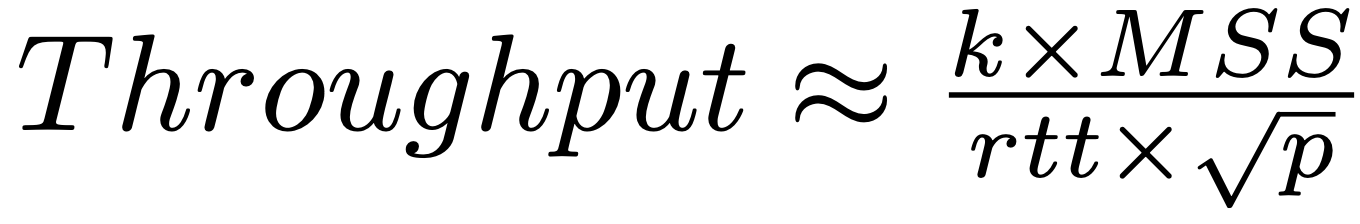
\includegraphics[width=0.3\textwidth]{Capture4.png}
    %\caption{}
\end{solfig}

Débit A: $\frac{k \cdot MSS}{25 \cdot \sqrt{10/1000}} = \frac{k \cdot MSS}{2.5}$\\

Débit B: $\frac{k \cdot MSS}{20 \cdot \sqrt{20/1000}} = \frac{k \cdot MSS}{2.828}$\\

Débit C: $\frac{k \cdot MSS}{30 \cdot \sqrt{5/1000}} = \frac{k \cdot MSS}{2.121}$\\

Si le MSS est équivalent pour toute les connexions alors la connexion C aura le plus grand débit.\\

$\frac{k}{2.121} > \frac{k}{2.5} > \frac{k}{2.828}$ 
\end{solution}


\section{TCP [2 points]}
Le protocole TCP fonctionne en mode bytestream et fournit un service fiable. Comment le modifieriez-vous de façon à ce qu'il fonctionne en mode message et puisse supporter des messages dont la taille est comprise entre 1 et $2^{30}$ octets ? Vous pouvez changer le format de l'entête TCP si vous le souhaitez.

\begin{solution}
Monsieur OBO a dit qu'il ne fallait pas connaître de théorie pour cette question, mais qu'il faut pouvoir se débrouiller un peu avec ce qui sort un peu du cours et être créatif... À votre tour j'ai envie de dire ;p 
\end{solution}

\section{TLS et ssh [1 point]}
Les protocoles ssh et TLS que nous avons étudié dans le cours utilisent des techniques cryp-tographiques pour s'assurer de la confidentialité des échanges entre un client et un serveur. Une des différences importantes entre ces deux protocoles est la façon dont le client authentifie le serveur avec lequel il interagit. Expliquez les stratégies choisies par ssh et TLS et justifiez pourquoi à votre avis la solution utilisée par ssh n'est pas utilisée par TLS pour sécuriser HTTPS et vice-versa.

\begin{solution}
Le serveur ssh n'envoie pas de certificat. Il fait l'hypothèse que le client le connaît déjà, et possède dans sa cache la clé publique des serveurs au quels il se connecte habituellement. Si ce n'est pas le cas, le serveur envoie alors sa clé publique, mais il n'est pas possible pour le client d'authentifier le serveur. C'est inadmissible en HTTP, tant au point de vu sécuritaire qu'au point de vue du stockage. En effet, si on retient les clé de tout les sites web que l'on visite, on utilise de la mémoire inutilement.
\end{solution}


\section{HTTP/1.1 et HTTP/2.0 [1 point]}
Quelles sont les différences principales entre HTTP/1.1 et HTTP/2.0 ?

\begin{solution}
\begin{itemize}
\item Multiplexing
\item Piplining
\item et bien plus encore
%je vous invite à en rajouter ou à les décrire ;)
\item server push
\item encodage des données en binaire
\end{itemize}
\end{solution}

\section{traceroute [2 points]}
Le réseau ci-dessous contient six routeurs, Ri, R2,R3,R4, R5 et R6 et deux hôtes.
\begin{center}
    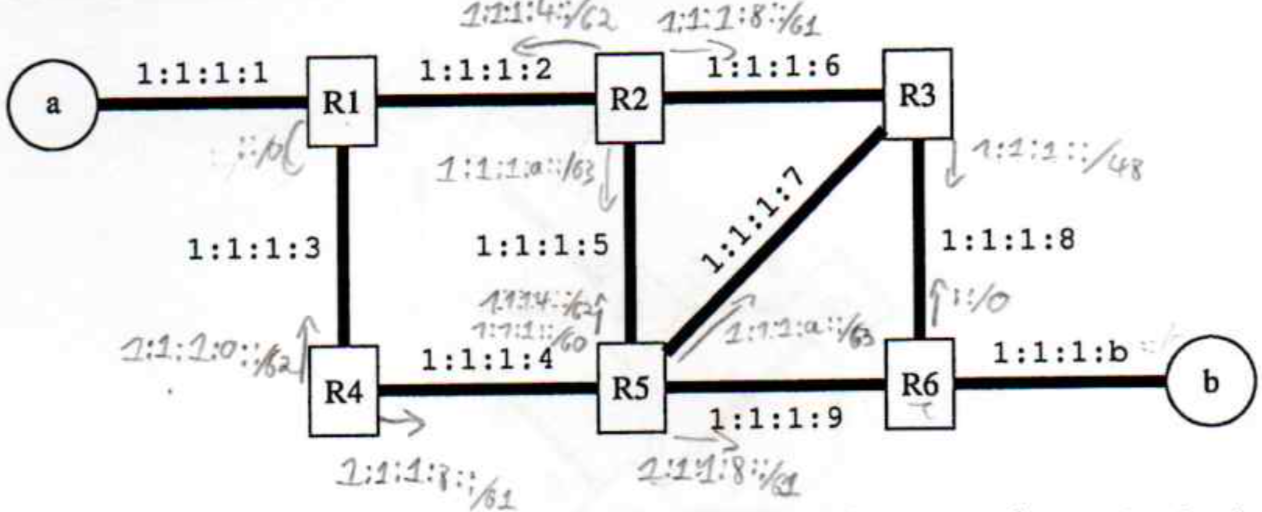
\includegraphics[width=0.7\linewidth]{Capture.png}
\end{center}
Les sous-réseaux sur la figure sont tous des /64. Dans le sous-réseau 1:1:1:2, le routeur R2 a comme adresse 1:1:1:2::2/64, R1 1:1:1:2::1/64. L'hôte \textit{b} a comme adresse 1:1:1:b::b/64. L'hôte \textit{a} a comme adresse 1:1:1:1::a/64. Chaque routeur connait évidemment tous les sous-réseaux auxquels il est directement connecté. De plus, les routes statiques suivantes sont configurées:
\begin{itemize}
    \item Sur R1: ::/0 via 1:1:1:3::4 
    \item Sur R2: 1:1:1:a::/63 via 1:1:1:5::5 , 1:1:1:8::1/61 via 1:1:1:6::3 et 1:1:1:4::/62 via 1:1:1:2::1
    \item Sur R3: 1:1:1::/48 via 1:1:1:8::6
    \item Sur R4: 1:1:1:8::/61 via 1:1:1:4::5 , 1:1:1:0::/62 via 1:1:1:3::1
    \item Sur R5: 1:1:1:8::/61 via 1:1:1:9::6, 1:1:1:4::/62 via 1:1:1:5::2, 1:1:1:a::/63 via 1:1:1:7::3 et 1:1:1::/60 via 1:1:1:5::2
    \item Sur R6 ::/0 via 1:1:1:8::3 
\end{itemize}
\begin{enumerate}
    \item Sur base de ces tables de routage, déterminez précisément le chemin suivi par un paquet envoyé par R5 à destination de b. Représentez ce chemin sous la forme d'une liste de routeurs, comme R5-R9-R7-... et justifiez brièvement votre réponse.
    \item Même question pour le chemin de R6 vers a
    \item Même question pour le chemin de a vers b
    \item Quel résultat donnerait traceroute  b lancé depuis a ? 
\end{enumerate}


\begin{solution}
\begin{enumerate}
\item R5-R3-R6-b car l'adresse de 'b' matche avec la route "/63" du serveur R5. En effet, en binaire, 'a' correspond à 1010 et le 'b' à 1011.
\item R6-R3-R6-R3-$\cdots$
\item a-R1-R4-R5-R3-R6-b
\item Le premier hop retourne l'adresse 1:1:1:1::1. Les hops suivant ne retournent rien, en effet il n'y a pas de route a partir de [R4, R5, R3, R6] vers l'hôte a.  
\end{enumerate}
\end{solution}

\section{Spanning Tree [2 points] }
Le réseau ci-dessous contient six switches, S1, S2, S3, S4, S5 et S6. 
\begin{center}
    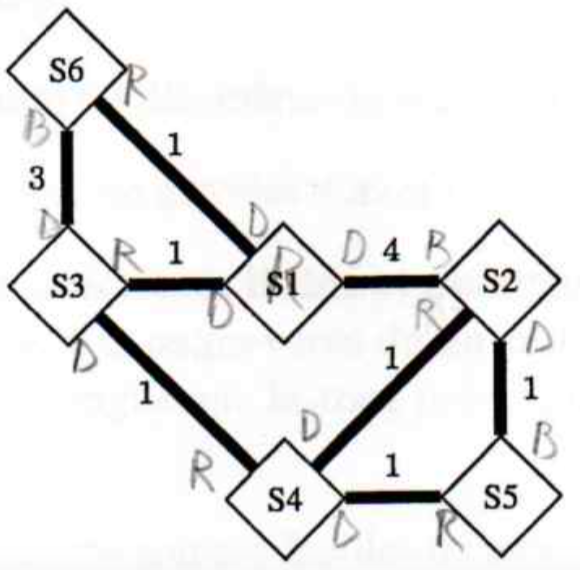
\includegraphics[width=0.5\linewidth]{Capture2.png}
\end{center}
Dans ce reseau Ethernet, quelles sont les interfaces des switches qui seront dans l'état bloque? Si l'interface de S1 vers S3 est bloquée, indiquez S1$\rightarrow$S3.

\begin{solution}
$S6\rightarrow S3$

$S2\rightarrow S1$

$S5\rightarrow S2$
\end{solution}

\section{BGP [2 points]}
Dans le reseau ci-dessous, AS1 annonce le préfixe pl et AS 8 le préfixe p8. Les flèches dirigées indiquent les relations customer-provider (du customer vers le provider) et les lignes avec le signe = les relations shared-cost.
\begin{center}
    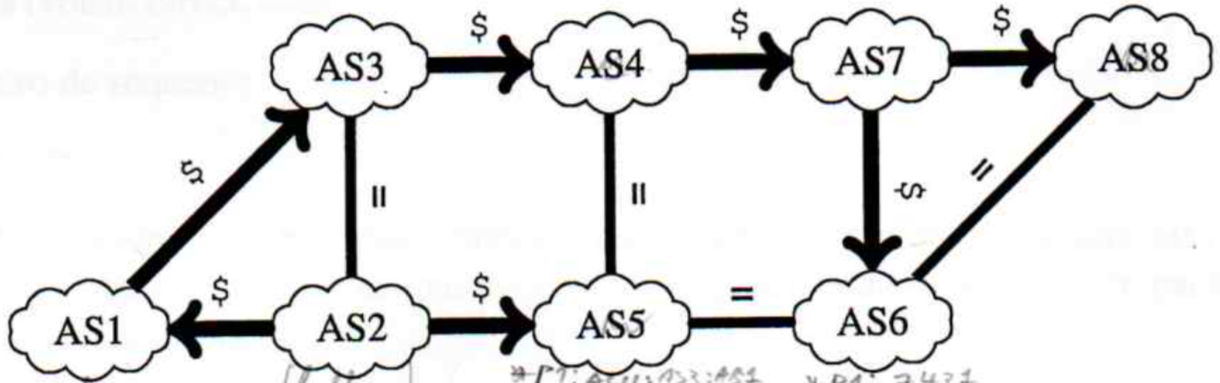
\includegraphics[width=0.6\linewidth]{Capture3.png}
\end{center}
\begin{itemize}
    \item Quelle est la table de routage complète de AS 4 pour le préfixe pl annonce par AS 1 (indiquez avec une étoile la route préférée) ? 
    \item Quelle est la table de routage complète de AS 8 pour le préfixe pl annonce par AS 1 (indiquez avec une étoile la route préférée) ?
    \item Quelle est la table de routage complète de AS 5 pour le préfixe pl annonce par AS 1 (indiquez avec une étoile la route préférée)?
\end{itemize}

\begin{solution}

\begin{enumerate}
\item * P1;AS3:AS1
\item * P1;AS7:AS4:AS3:AS1\\
P1;AS6:AS7:AS4:AS3:AS1
\item *P1;AS4:AS3:AS1\\
P1;AS6:AS7:AS4:AS3:AS1
\end{enumerate}

Une des difficulté de cet exercice est de bien se rappeler que l'on envoie que les meilleures routes (du point de vue du routeur). La route préférée sera toujours choisie selon les critères: Relation sur lien (client,shared-cost-provider) puis la longueur.
\end{solution}

\end{document}
